\documentclass[a4paper, 12pt]{article}
\usepackage[T1]{fontenc}
\usepackage[utf8]{inputenc}
\usepackage{booktabs}
\usepackage{titling}
\usepackage{titlesec}
\usepackage{amssymb}
\usepackage{pifont}
\usepackage{graphicx}
\graphicspath{ {../../} }

\usepackage{hyperref}
\hypersetup{
    colorlinks=true,
    linkcolor=black,
    % filecolor=magenta,
    urlcolor=cyan,
}
\urlstyle{same}

\newcommand{\cmark}{\ding{51}}
\newcommand{\xmark}{\ding{55}}

\renewcommand{\contentsname}{Obsah}
% \renewcommand{\thesection}{\Roman{section}.}
\renewcommand{\thesection}{\Roman{section}}
\renewcommand{\thesubsection}{\roman{subsection}}

\titleformat{\section}
{\Large\bfseries}
% {\Roman{section}.}
{\thesection}
{0.5em}
{}


\titleformat{\subsection}
{\large\bfseries}
{\thesubsection.}
{0.5em}
{}

\title{
        \vspace{1in}
        \rule{\linewidth}{0.5pt}
		\usefont{OT1}{bch}{b}{n}
        \huge Uživatelská dokumentace \\GrainSim\\
        \vspace{-10pt}
        \rule{\linewidth}{1pt}
}
\author{
		\normalfont\normalsize
        Marek Bečvář\\[-3pt]\normalsize
        31.7.2021
}
\date{}



\begin{document}
\maketitle 
\newpage

\tableofcontents
\newpage

\section{O programu} 
\paragraph{}
GrainSim je fyzikální sandbox, ve kterém uživatel může experimentovat s řadou 
prvků. Vlastnosti těchto prvků (teploty tuhnutí, tání, hořlavost, výbušnost, rychlost
přenosu tepla) jsou založené v jejich předlohách z reálného světa.

Uživatel má pak k dispozici herní plochu, do která může vkládat libovolné z
dostupných prvků a dále i upravovat teplotu prostředí. To celá v 2D interaktivním 
znázornění herního prostředí.

\section{Spuštění/Kompilace}
\paragraph{C\#}
Projekt je vytvořen v C\# .NET Core 3.1 s využitím frameworku Monogame verze 3.8.
\url{https://www.monogame.net}. Projekt byl vytvářen v Linuxu. Jsou ale
přiložené verze kompatibilní jak s platformou Linux tak Windows (jediný rozdíl je, že verze
pro Linux umožňuje maximálně jeden uložený projekt/Win verze prakticky
nekonečno, přes file explorer).

\paragraph{Spuštění}
Pro spuštění programu není potřeba žádných dalších kroků, krom spuštění
přiloženého exe souboru.

\paragraph{Kompilace}
Pro kompilování zdrojového kódu je potřeba mít nainstalované NuGet balíčky framework
Monogame. Kód využívá balíčky \\\textbf{Monogame.Framework.DesktopGL} a
\\\textbf{Monogame.Content.Builder.Task} - obojí verze \textbf{3.8.0.1614}. 
Kompilace provedena v IDE Visual Studio 2019 - C\# .NET Core 3.1.

\newpage
\section{Herní prostředí}
\paragraph{Spuštění}
Pro spuštění programu je potřeba pouze spustit přiložený exe soubor.
Uživatel se octne na základní obrazovce, kde je ve vrchní části herní plocha a
ve spodní víceúrovňové menu.

\begin{center}
   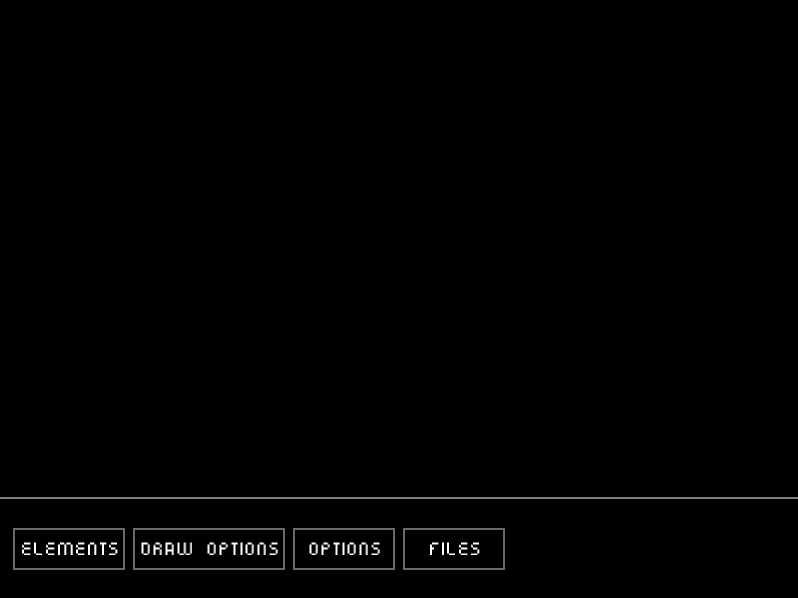
\includegraphics[width=0.9\linewidth]{img3.png}
\end{center}

\paragraph{Menu}
Menu obsahuje následující sekce:
\begin{itemize}
    \item \textbf{Elements}
    \subitem Solids, Liquids, Gasses, Specials
    \subsubitem Seznam jednotlivých použitelných prvků, dle kategorií 
\item \textbf{Draw Options}
    \subitem Alternativní možnosti vykreslování herní plochy
\item \textbf{Options}
    \subitem Nastavení umožnující vykreslovat dodatečné informace o stavu
    prostředí
\item \textbf{Files}
    \subitem Možnosti načítání a ukládání aktuálního prostředí

\end{itemize}
\newpage

\paragraph{Ovládání}
Aplikace se může celá ovládat myší. Menu sekci může uživatel procházet klasicky
svyužitím levého tlačítka myši. V herním prostředí je potom kurzor a velikost
kurzoru znázorněna vykresleným ukazatelem. Velikost kurzoru může uživatel měnit
buď kolečkem myši, nebo šipkami \\(šipka nahoru - zvětší kurzor,
šipka dolů - zmenší). Dále může uživatel přepínat mezi dvěma režimi vykreslování (zobrazení
částic/zobrazení teplot). \\To je možno provést přes tlačítka hlavního menu nebo
přes klávesy \\F1 (= částice) a F2 (= teploty).

\paragraph{}
V herním prostředí (oblast nad menu) je pak vždy levé tlačítko myši přidávání
právě vybraného prvku do prostředí a levé tlačíko mazání prvků v oblasti pod
kurzorem. 

\paragraph{}
V celé aplikaci platí, že tlačítko \textbf{Escape} může být použito k \textbf{okamžitému
ukončení}.

\paragraph{Ukládání}
\textbf{Ve verzi pro Windows} má uživatel možnost kdykoliv uložit aktuální stav 
herního prostředí a to přes tlačítka hlavní sekci menu. Po stisknutí tlačítka
\textbf{Save Project}/\textbf{Load Project} se otevře prohlížeč souborů, kde
může uživatel vybrat umístění a jméno kam svoji simulaci uložit/odkud ji
nahrát. \\
Soubory (\emph{*.grain}) jsou ukládány jako kolekce dat ze simulačního prostředí převedena do
binární podoby. Proces ukládání je díky tomu bezztrátový. Po načtení se tedy
prostředí uvede do podoby totožné s momentem, kdy bylo dříve uloženo.

\paragraph{!}
\textbf{Ve verzi pro Linux} je momentálně možno ukládat pouze jedno prostředí a
opakované ukládání bude přepisovat poslední záznam.

\section{Závěr}
Projekt byl vytvoření jako záverečná semestrální práce pro předmět
\\\emph{Programování 2} - Letní semestr 2021 - UK Matfyz.
\end{document}
